\documentclass[UTF8,fntef,a4paper]{article}
\usepackage{graphicx}
\usepackage{amsmath,amssymb}
\usepackage{savesym}
\usepackage{amscd}
\usepackage{latexsym}
\usepackage{arydshln,multirow}
\usepackage{listings} 
\usepackage{xcolor}
\usepackage{graphicx} 
\usepackage{CJK}
\makeatletter %使\section中的内容左对齐
\renewcommand{\section}{\@startsection{section}{1}{0mm}
  {1.5\baselineskip}{0.5\baselineskip}{\bf\leftline}}
\newcommand{\tabincell}[2]{\begin{tabular}{@{}#1@{}}#2\end{tabular}}
\makeatother
\begin{document}
\begin{CJK*}{UTF8}{kai}
\title{\Large 计算机系统综合实验}
\author{计33~ ~伍一鸣~ ~2012011347}
\maketitle
\tableofcontents
\newpage
\section{实验目标及完成情况}
	\subsection{实验目标}
	实现32位mips指令系统的五级流水线CPU,在CPU上运行监控程序。
	\subsection{完成情况}
	完成了32位mips指令系统的五级流水线CPU,未能运行监控程序,在CPU上运行了一个fibonacci数列计算的程序。
	
\section{项目分工}
	\begin{itemize}
	\item 设计数据通路和指令集:杜华峰,郭栋,伍一鸣
	\item CPU代码实现与调试:杜华峰,郭栋
	\item 监控程序的修改:伍一鸣
	\item 所有文档撰写:伍一鸣
	\end{itemize}
\newpage

\section{指令机器码}
rd,rs,rt均为寄存器
\subsection{逻辑操作}
	\begin{table}[!hbp]
		\centering
		\begin{tabular}{|c|c|c|c|c|c|c|}
		\hline
		\multirow{2}{*}{指令编码} & 31-26&25-21 & 20-16&15-11 &10-6 &5-0\\
		\cline{2-7} & 000000 & rs & rt & rd & 00000 & 100100 \\
		\hline
		指令格式&\multicolumn{6}{|l|}{AND rd rs rt}\\
		\hline		
		指令功能&\multicolumn{6}{|l|}{R[d] $\leftarrow$ R[s] \& R[t]}\\
		\hline		
		功能说明&\multicolumn{6}{|l|}{将rs 与rt 的值相与后的结果保存至rd 中}\\
		\hline
		\end{tabular}
	\end{table}
	\begin{table}[!hbp]
		\centering
		\begin{tabular}{|c|c|c|c|c|c|c|}
		\hline
		\multirow{2}{*}{指令编码} & 31-26&25-21 & 20-16&15-11 &10-6 &5-0\\
		\cline{2-7} & 000000 & rs & rt & rd & 00000 & 100101 \\
		\hline
		指令格式&\multicolumn{6}{|l|}{OR rd rs rt}\\
		\hline		
		指令功能&\multicolumn{6}{|l|}{R[d] $\leftarrow$ R[s] $|$ R[t]}\\
		\hline		
		功能说明&\multicolumn{6}{|l|}{将rs 与rt 的值相或后的结果保存至rd 中}\\
		\hline
		\end{tabular}
	\end{table}
	\begin{table}[!hbp]
		\centering
		\begin{tabular}{|c|c|c|c|c|c|c|}
		\hline
		\multirow{2}{*}{指令编码} & 31-26&25-21 & 20-16&15-11 &10-6 &5-0\\
		\cline{2-7} & 000000 & rs & rt & rd & 00000 & 100110 \\
		\hline
		指令格式&\multicolumn{6}{|l|}{XOR rd rs rt}\\
		\hline		
		指令功能&\multicolumn{6}{|l|}{R[d] $\leftarrow$ R[s] $\land$ R[t]}\\
		\hline		
		功能说明&\multicolumn{6}{|l|}{将rs 与rt 的值相异或后的结果保存至rd 中}\\
		\hline
		\end{tabular}
	\end{table}
	\begin{table}[!hbp]
		\centering
		\begin{tabular}{|c|c|c|c|c|c|c|}
		\hline
		\multirow{2}{*}{指令编码} & 31-26&25-21 & 20-16&15-11 &10-6 &5-0\\
		\cline{2-7} & 000000 & rs & rt & rd & 00000 & 100111 \\
		\hline
		指令格式&\multicolumn{6}{|l|}{NOR rd rs rt}\\
		\hline		
		指令功能&\multicolumn{6}{|l|}{R[d] $\leftarrow \sim$(R[s] $|$ R[t])}\\
		\hline		
		功能说明&\multicolumn{6}{|l|}{将rs 与rt 的值或非后的结果保存至rd 中}\\
		\hline
		\end{tabular}
	\end{table}
\newpage

	\begin{table}[!hbp]
		\centering
		\begin{tabular}{|c|c|c|c|c|c|c|}
		\hline
		\multirow{2}{*}{指令编码} & 31-26&25-21 & 20-16&15-11 &10-6 &5-0\\
		\cline{2-7} & 001100 & rs & rt & \multicolumn{3}{|c|}{immediate} \\
		\hline
		指令格式&\multicolumn{6}{|l|}{ANDI rt rs immediate}\\
		\hline		
		指令功能&\multicolumn{6}{|l|}{R[t] $\leftarrow$  R[s] \& Zero-extend(immediate)}\\
		\hline		
		功能说明&\multicolumn{6}{|l|}{将 rs 的值与立即数零扩展后相与的结果保存至rt 中}\\
		\hline
		\end{tabular}
	\end{table}
	\begin{table}[!hbp]
		\centering
		\begin{tabular}{|c|c|c|c|c|c|c|}
		\hline
		\multirow{2}{*}{指令编码} & 31-26&25-21 & 20-16&15-11 &10-6 &5-0\\
		\cline{2-7} & 001110 & rs & rt & \multicolumn{3}{|c|}{immediate} \\
		\hline
		指令格式&\multicolumn{6}{|l|}{XORI rt rs immediate}\\
		\hline		
		指令功能&\multicolumn{6}{|l|}{R[t] $\leftarrow$  R[s] $\land$ Zero-extend(immediate)}\\
		\hline		
		功能说明&\multicolumn{6}{|l|}{将 rs 的值与立即数零扩展后相异或的结果保存至rt 中}\\
		\hline
		\end{tabular}
	\end{table}
	\begin{table}[!hbp]
		\centering
		\begin{tabular}{|c|c|c|c|c|c|c|}
		\hline
		\multirow{2}{*}{指令编码} & 31-26&25-21 & 20-16&15-11 &10-6 &5-0\\
		\cline{2-7} & 001111 & 00000 & rt & \multicolumn{3}{|c|}{immediate} \\
		\hline
		指令格式&\multicolumn{6}{|l|}{LUI rt immediate}\\
		\hline		
		指令功能&\multicolumn{6}{|l|}{R[t] $\leftarrow$   immediate * 65536}\\
		\hline		
		功能说明&\multicolumn{6}{|l|}{将 16 位立即数放至 rt 的高 16 位中}\\
		\hline
		\end{tabular}
	\end{table}
	\begin{table}[!hbp]
		\centering
		\begin{tabular}{|c|c|c|c|c|c|c|}
		\hline
		\multirow{2}{*}{指令编码} & 31-26&25-21 & 20-16&15-11 &10-6 &5-0\\
		\cline{2-7} & 001101 & rs & rt & \multicolumn{3}{|c|}{immediate} \\
		\hline
		指令格式&\multicolumn{6}{|l|}{ORI rt rs immediate}\\
		\hline		
		指令功能&\multicolumn{6}{|l|}{R[t] $\leftarrow$  R[s] $|$ Zero-extend(immediate)}\\
		\hline		
		功能说明&\multicolumn{6}{|l|}{将 rs 与立即数 immediate 零扩展后相或的结果保存至rd 中}\\
		\hline
		\end{tabular}
	\end{table}
\newpage

\subsection{移位操作}
	\begin{table}[!hbp]
		\centering
		\begin{tabular}{|c|c|c|c|c|c|c|}
		\hline
		\multirow{2}{*}{指令编码} & 31-26&25-21 & 20-16&15-11 &10-6 &5-0\\
		\cline{2-7} & 000000 & 00000 & rt & rd & immediate& 000000 \\
		\hline
		指令格式&\multicolumn{6}{|l|}{SLL rd rt immediate}\\
		\hline		
		指令功能&\multicolumn{6}{|l|}{R[d] $\leftarrow$  R[t] $<<$ immediate}\\
		\hline		
		功能说明&\multicolumn{6}{|l|}{将 rt 中的值左移立即数 immediate 位后的结果保存至 rd 中}\\
		\hline
		\end{tabular}
	\end{table}
	\begin{table}[!hbp]
		\centering
		\begin{tabular}{|c|c|c|c|c|c|c|}
		\hline
		\multirow{2}{*}{指令编码} & 31-26&25-21 & 20-16&15-11 &10-6 &5-0\\
		\cline{2-7} & 000000 & 00000 & rt & rd & immediate& 000010 \\
		\hline
		指令格式&\multicolumn{6}{|l|}{SRL rd rt immediate}\\
		\hline		
		指令功能&\multicolumn{6}{|l|}{R[d] $\leftarrow$  R[t] $>>$ immediate(logical)}\\
		\hline		
		功能说明&\multicolumn{6}{|l|}{将 rt 中的值逻辑右移立即数 immediate 位后的结果保存至 rd 中}\\
		\hline
		\end{tabular}
	\end{table}
	\begin{table}[!hbp]
		\centering
		\begin{tabular}{|c|c|c|c|c|c|c|}
		\hline
		\multirow{2}{*}{指令编码} & 31-26&25-21 & 20-16&15-11 &10-6 &5-0\\
		\cline{2-7} & 000000 & 00000 & rt & rd & immediate& 000011 \\
		\hline
		指令格式&\multicolumn{6}{|l|}{SRA rd rt immediate}\\
		\hline		
		指令功能&\multicolumn{6}{|l|}{R[d] $\leftarrow$  R[t] $>>$ immediate(arithmetic)}\\
		\hline		
		功能说明&\multicolumn{6}{|l|}{将 rt 中的值算术右移立即数 immediate 位后的结果保存至 rd 中}\\
		\hline
		\end{tabular}
	\end{table}
\newpage

	\begin{table}[!hbp]
		\centering
		\begin{tabular}{|c|c|c|c|c|c|c|}
		\hline
		\multirow{2}{*}{指令编码} & 31-26&25-21 & 20-16&15-11 &10-6 &5-0\\
		\cline{2-7} & 000000 & rs & rt & rd & 00000& 000100 \\
		\hline
		指令格式&\multicolumn{6}{|l|}{SLLV rd rt rs}\\
		\hline		
		指令功能&\multicolumn{6}{|l|}{R[d] $\leftarrow$  R[t] $<<$ R[s]}\\
		\hline		
		功能说明&\multicolumn{6}{|l|}{将 rt 中的值左移 rs 位后的结果保存至 rd 中}\\
		\hline
		\end{tabular}
	\end{table}
	\begin{table}[!hbp]
		\centering
		\begin{tabular}{|c|c|c|c|c|c|c|}
		\hline
		\multirow{2}{*}{指令编码} & 31-26&25-21 & 20-16&15-11 &10-6 &5-0\\
		\cline{2-7} & 000000 & rs & rt & rd & 00000& 000110 \\
		\hline
		指令格式&\multicolumn{6}{|l|}{SRLV rd rt rs}\\
		\hline		
		指令功能&\multicolumn{6}{|l|}{R[d] $\leftarrow$  R[t] $>>$ R[s](logical)}\\
		\hline		
		功能说明&\multicolumn{6}{|l|}{将 rt 中的值逻辑右移rs 位后的结果保存至 rd 中}\\
		\hline
		\end{tabular}
	\end{table}
	\begin{table}[!hbp]
		\centering
		\begin{tabular}{|c|c|c|c|c|c|c|}
		\hline
		\multirow{2}{*}{指令编码} & 31-26&25-21 & 20-16&15-11 &10-6 &5-0\\
		\cline{2-7} & 000000 & rs & rt & rd & 00000& 000111 \\
		\hline
		指令格式&\multicolumn{6}{|l|}{SRAV rd rt rs}\\
		\hline		
		指令功能&\multicolumn{6}{|l|}{R[d] $\leftarrow$  R[t] $>>$ R[s](arithmetic)}\\
		\hline		
		功能说明&\multicolumn{6}{|l|}{将 rt 中的值算术右移rs位后的结果保存至 rd 中}\\
		\hline
		\end{tabular}
	\end{table}
\newpage

\subsection{移动操作}
	\begin{table}[!hbp]
		\centering
		\begin{tabular}{|c|c|c|c|c|c|c|}
		\hline
		\multirow{2}{*}{指令编码} & 31-26&25-21 & 20-16&15-11 &10-6 &5-0\\
		\cline{2-7} & 000000 & rs & rt & rd & 00000& 001011 \\
		\hline
		指令格式&\multicolumn{6}{|l|}{MOVN rd rt rs}\\
		\hline		
		指令功能&\multicolumn{6}{|l|}{if rt $\neq$ 0 then rd $\leftarrow$ rs}\\
		\hline		
		功能说明&\multicolumn{6}{|l|}{若rt不为0,则将rs的值赋给rd}\\
		\hline
		\end{tabular}
	\end{table}
	\begin{table}[!hbp]
		\centering
		\begin{tabular}{|c|c|c|c|c|c|c|}
		\hline
		\multirow{2}{*}{指令编码} & 31-26&25-21 & 20-16&15-11 &10-6 &5-0\\
		\cline{2-7} & 000000 & rs & rt & rd & 00000& 001010 \\
		\hline
		指令格式&\multicolumn{6}{|l|}{MOVZ rd rt rs}\\
		\hline		
		指令功能&\multicolumn{6}{|l|}{if rt = 0 then rd $\leftarrow$ rs}\\
		\hline		
		功能说明&\multicolumn{6}{|l|}{若rt为0,则将rs的值赋给rd}\\
		\hline
		\end{tabular}
	\end{table}
\newpage

\subsection{算术操作}
	\begin{table}[!hbp]
		\centering
		\begin{tabular}{|c|c|c|c|c|c|c|}
		\hline
		\multirow{2}{*}{指令编码} & 31-26&25-21 & 20-16&15-11 &10-6 &5-0\\
		\cline{2-7} & 000000 & rs & rt & rd & 00000 & 100001 \\
		\hline
		指令格式&\multicolumn{6}{|l|}{ADDU rd rs rt}\\
		\hline		
		指令功能&\multicolumn{6}{|l|}{R[d] $\leftarrow$ R[s] + R[t]}\\
		\hline		
		功能说明&\multicolumn{6}{|l|}{将rs 与rt 的值相加后的结果保存至rd 中}\\
		\hline
		\end{tabular}
	\end{table}
	\begin{table}[!hbp]
		\centering
		\begin{tabular}{|c|c|c|c|c|c|c|}
		\hline
		\multirow{2}{*}{指令编码} & 31-26&25-21 & 20-16&15-11 &10-6 &5-0\\
		\cline{2-7} & 000000 & rs & rt & rd & 00000 & 100011 \\
		\hline
		指令格式&\multicolumn{6}{|l|}{SUBU rd rs rt}\\
		\hline		
		指令功能&\multicolumn{6}{|l|}{R[d] $\leftarrow$ R[s] - R[t]}\\
		\hline		
		功能说明&\multicolumn{6}{|l|}{将rs 与rt 的值相减后的结果保存至rd 中}\\
		\hline
		\end{tabular}
	\end{table}
	\begin{table}[!hbp]
		\centering
		\begin{tabular}{|c|c|c|c|c|c|c|}
		\hline
		\multirow{2}{*}{指令编码} & 31-26&25-21 & 20-16&15-11 &10-6 &5-0\\
		\cline{2-7} & 000000 & rs & rt & rd & 00000 & 101010 \\
		\hline
		指令格式&\multicolumn{6}{|l|}{SLT rd rs rt}\\
		\hline		
		指令功能&\multicolumn{6}{|l|}{if(R[s] $<$ R[t]) then R[d] = 1,else R[d] = 0}\\
		\hline		
		功能说明&\multicolumn{6}{|l|}{比较 rs 与 rt 的值并根据结果将 rd 赋值}\\
		\hline
		\end{tabular}
	\end{table}
	\begin{table}[!hbp]
		\centering
		\begin{tabular}{|c|c|c|c|c|c|c|}
		\hline
		\multirow{2}{*}{指令编码} & 31-26&25-21 & 20-16&15-11 &10-6 &5-0\\
		\cline{2-7} & 000000 & rs & rt & rd & 00000 & 101011 \\
		\hline
		指令格式&\multicolumn{6}{|l|}{SLTU rd rs rt}\\
		\hline		
		指令功能&\multicolumn{6}{|l|}{if(R[s] $<$ R[t]) then R[d] = 1,else R[d] = 0}\\
		\hline		
		功能说明&\multicolumn{6}{|l|}{比较 rs 与 rt 的无符号值并根据结果将 rd 赋值}\\
		\hline
		\end{tabular}
	\end{table}
\newpage

	\begin{table}[!hbp]
		\centering
		\begin{tabular}{|c|c|c|c|c|c|c|}
		\hline
		\multirow{2}{*}{指令编码} & 31-26&25-21 & 20-16&15-11 &10-6 &5-0\\
		\cline{2-7} & 001001 & rs & rt & \multicolumn{3}{|c|}{immediate} \\
		\hline
		指令格式&\multicolumn{6}{|l|}{ADDIU rt rs immediate}\\
		\hline		
		指令功能&\multicolumn{6}{|l|}{R[t] $\leftarrow$ R[s] + (sign extended)immediate}\\
		\hline		
		功能说明&\multicolumn{6}{|l|}{对立即数immediate进行符号扩展后与rs的值求和,保存到rt中,不检查溢出}\\
		\hline
		\end{tabular}
	\end{table}
	\begin{table}[!hbp]
		\centering
		\begin{tabular}{|c|c|c|c|c|c|c|}
		\hline
		\multirow{2}{*}{指令编码} & 31-26&25-21 & 20-16&15-11 &10-6 &5-0\\
		\cline{2-7} & 001010 & rs & rt & \multicolumn{3}{|c|}{immediate} \\
		\hline
		指令格式&\multicolumn{6}{|l|}{SLTI rt rs immediate}\\
		\hline		
		指令功能&\multicolumn{6}{|l|}{if( R[s] $<$ (sign extended)immediate )then R[t]=1,else R[t]=0}\\
		\hline		
		功能说明&\multicolumn{6}{|l|}{对立即数immediate进行符号扩展后与rs的值无符号比较并根据结果将 rt 赋值}\\
		\hline
		\end{tabular}
	\end{table}
	\begin{table}[!hbp]
		\centering
		\begin{tabular}{|c|c|c|c|c|c|c|}
		\hline
		\multirow{2}{*}{指令编码} & 31-26&25-21 & 20-16&15-11 &10-6 &5-0\\
		\cline{2-7} & 001011 & rs & rt & \multicolumn{3}{|c|}{immediate} \\
		\hline
		指令格式&\multicolumn{6}{|l|}{SLTIU rt rs immediate}\\
		\hline		
		指令功能&\multicolumn{6}{|l|}{if( R[s] $<$ (sign extended)immediate )then R[t]=1,else R[t]=0}\\
		\hline		
		功能说明&\multicolumn{6}{|l|}{对立即数immediate进行符号扩展后与rs的值有符号比较并根据结果将 rt 赋值}\\
		\hline
		\end{tabular}
	\end{table}
\newpage

\subsection{转移指令}
	\begin{table}[!hbp]
		\centering
		\begin{tabular}{|c|c|c|c|c|c|c|}
		\hline
		\multirow{2}{*}{指令编码} & 31-26&25-21 & 20-16&15-11 &10-6 &5-0\\
		\cline{2-7} & 000000 & rs & 00000 & 00000& 00000& 001000 \\
		\hline
		指令格式&\multicolumn{6}{|l|}{JR rs}\\
		\hline		
		指令功能&\multicolumn{6}{|l|}{PC $\leftarrow$ R[s]}\\
		\hline		
		功能说明&\multicolumn{6}{|l|}{无条件跳转至 rs 中所存地址执行}\\
		\hline
		\end{tabular}
	\end{table}
	\begin{table}[!hbp]
		\centering
		\begin{tabular}{|c|c|c|c|c|c|c|}
		\hline
		\multirow{2}{*}{指令编码} & 31-26&25-21 & 20-16&15-11 &10-6 &5-0\\
		\cline{2-7} & 000000 & rs & 00000 & rd& 00000& 001001 \\
		\hline
		指令格式&\multicolumn{6}{|l|}{JALR rd rs 或者JALR rs}\\
		\hline		
		指令功能&\multicolumn{6}{|l|}{PC $\leftarrow$ R[s], R[d] $\leftarrow$ RPC}\\
		\hline		
		功能说明&\multicolumn{6}{|l|}{\tabincell{c}{无条件跳转至 rs 中所存地址执行,将延时槽后一条指令\\的地址保存到 rd中作为返回地址,rd默认为\$31}}\\
		\hline
		\end{tabular}
	\end{table}
	\begin{table}[!hbp]
		\centering
		\begin{tabular}{|c|c|c|c|c|c|c|}
		\hline
		\multirow{2}{*}{指令编码} & 31-26&25-21 & 20-16&15-11 &10-6 &5-0\\
		\cline{2-7} & 000010 & \multicolumn{5}{|c|}{instr index} \\
		\hline
		指令格式&\multicolumn{6}{|l|}{J target}\\
		\hline		
		指令功能&\multicolumn{6}{|l|}{PC $\leftarrow$ (PC+4)[31,28]$||$target*4}\\
		\hline		
		功能说明&\multicolumn{6}{|l|}{\tabincell{c}{跳转至新地址执行,新地址低28位为target乘以4的值,\\新地址高4位为PC+4的高4位}}\\
		\hline
		\end{tabular}
	\end{table}
	\begin{table}[!hbp]
		\centering
		\begin{tabular}{|c|c|c|c|c|c|c|}
		\hline
		\multirow{2}{*}{指令编码} & 31-26&25-21 & 20-16&15-11 &10-6 &5-0\\
		\cline{2-7} & 000011 & \multicolumn{5}{|c|}{instr index} \\
		\hline
		指令格式&\multicolumn{6}{|l|}{JAL target}\\
		\hline		
		指令功能&\multicolumn{6}{|l|}{PC $\leftarrow$ (PC+4)[31,28]$||$target*4,\$31 $\leftarrow$ RPC}\\
		\hline		
		功能说明&\multicolumn{6}{|l|}{\tabincell{c}{跳转至新地址执行,新地址低28位为target乘以4的值,\\新地址高4位为PC+4的高4位,返回地址保存到\$31中}}\\
		\hline
		\end{tabular}
	\end{table}
	
	
	以上四条指令都要在转移之前先执行延迟槽指令
\newpage

	\begin{table}[!hbp]
		\centering
		\begin{tabular}{|c|c|c|c|c|c|c|}
		\hline
		\multirow{2}{*}{指令编码} & 31-26&25-21 & 20-16&15-11 &10-6 &5-0\\
		\cline{2-7} & 000100 & rs & rt & \multicolumn{3}{|c|}{offset} \\
		\hline
		指令格式&\multicolumn{6}{|l|}{BEQ rs rt offset}\\
		\hline		
		指令功能&\multicolumn{6}{|l|}{if (rs = rt) then PC = PC+4+(signed extend(offset * 4))}\\
		\hline		
		功能说明&\multicolumn{6}{|l|}{若rs等于rt则执行跳转操作}\\
		\hline
		\end{tabular}
	\end{table}
%	\begin{table}[!hbp]
%		\centering
%		\begin{tabular}{|c|c|c|c|c|c|c|}
%		\hline
%		\multirow{2}{*}{指令编码} & 31-26&25-21 & 20-16&15-11 &10-6 &5-0\\
%		\cline{2-7} & 000100 & 00000 & 00000 & \multicolumn{3}{|c|}{offset} \\
%		\hline
%		指令格式&\multicolumn{6}{|l|}{B offset}\\
%		\hline		
%		指令功能&\multicolumn{6}{|l|}{PC = PC+4+(signed extend(offset * 4))}\\
%		\hline		
%		功能说明&\multicolumn{6}{|l|}{无条件执行跳转操作}\\
%		\hline
%		\end{tabular}
%	\end{table}
	\begin{table}[!hbp]
		\centering
		\begin{tabular}{|c|c|c|c|c|c|c|}
		\hline
		\multirow{2}{*}{指令编码} & 31-26&25-21 & 20-16&15-11 &10-6 &5-0\\
		\cline{2-7} & 000111 & rs & 00000 & \multicolumn{3}{|c|}{offset} \\
		\hline
		指令格式&\multicolumn{6}{|l|}{BGTZ rs offset}\\
		\hline		
		指令功能&\multicolumn{6}{|l|}{if (rs $>$ 0) then PC = PC+4+(signed extend(offset * 4))}\\
		\hline		
		功能说明&\multicolumn{6}{|l|}{若rs大于0则执行跳转操作}\\
		\hline
		\end{tabular}
	\end{table}
	\begin{table}[!hbp]
		\centering
		\begin{tabular}{|c|c|c|c|c|c|c|}
		\hline
		\multirow{2}{*}{指令编码} & 31-26&25-21 & 20-16&15-11 &10-6 &5-0\\
		\cline{2-7} & 000110 & rs & 00000 & \multicolumn{3}{|c|}{offset} \\
		\hline
		指令格式&\multicolumn{6}{|l|}{BLEZ rs offset}\\
		\hline		
		指令功能&\multicolumn{6}{|l|}{if (rs $\leq$ 0) then PC = PC+4+(signed extend(offset * 4))}\\
		\hline		
		功能说明&\multicolumn{6}{|l|}{若rs不大于0则执行跳转操作}\\
		\hline
		\end{tabular}
	\end{table}
%\newpage

	\begin{table}[!hbp]
		\centering
		\begin{tabular}{|c|c|c|c|c|c|c|}
		\hline
		\multirow{2}{*}{指令编码} & 31-26&25-21 & 20-16&15-11 &10-6 &5-0\\
		\cline{2-7} & 000101 & rs & rt & \multicolumn{3}{|c|}{offset} \\
		\hline
		指令格式&\multicolumn{6}{|l|}{BNE rs rt offset}\\
		\hline		
		指令功能&\multicolumn{6}{|l|}{if (rs $\neq$ rt) then PC = PC+4+(signed extend(offset * 4))}\\
		\hline		
		功能说明&\multicolumn{6}{|l|}{若rs不等于rt则执行跳转操作}\\
		\hline
		\end{tabular}
	\end{table}
	\begin{table}[!hbp]
		\centering
		\begin{tabular}{|c|c|c|c|c|c|c|}
		\hline
		\multirow{2}{*}{指令编码} & 31-26&25-21 & 20-16&15-11 &10-6 &5-0\\
		\cline{2-7} & 000001 & rs & 00000 & \multicolumn{3}{|c|}{offset} \\
		\hline
		指令格式&\multicolumn{6}{|l|}{BLTZ rs offset}\\
		\hline		
		指令功能&\multicolumn{6}{|l|}{if (rs $<$ 0) then PC = PC+4+(signed extend(offset * 4))}\\
		\hline		
		功能说明&\multicolumn{6}{|l|}{若rs小于0则执行跳转操作}\\
		\hline
		\end{tabular}
	\end{table}
	\begin{table}[!hbp]
		\centering
		\begin{tabular}{|c|c|c|c|c|c|c|}
		\hline
		\multirow{2}{*}{指令编码} & 31-26&25-21 & 20-16&15-11 &10-6 &5-0\\
		\cline{2-7} & 000001 & rs & 00001 & \multicolumn{3}{|c|}{offset} \\
		\hline
		指令格式&\multicolumn{6}{|l|}{BLEZ rs offset}\\
		\hline		
		指令功能&\multicolumn{6}{|l|}{if (rs $\geq$ 0) then PC = PC+4+(signed extend(offset * 4))}\\
		\hline		
		功能说明&\multicolumn{6}{|l|}{若rs不小于0则执行跳转操作}\\
		\hline
		\end{tabular}
	\end{table}
\newpage
\subsection{存储指令和空指令}
	\begin{table}[!hbp]
		\centering
		\begin{tabular}{|c|c|c|c|c|c|c|}
		\hline
		\multirow{2}{*}{指令编码} & 31-26&25-21 & 20-16&15-11 &10-6 &5-0\\
		\cline{2-7} & 100011 & base & rt & \multicolumn{3}{|c|}{offset} \\
		\hline
		指令格式&\multicolumn{6}{|l|}{LW rt offset(base)}\\
		\hline		
		指令功能&\multicolumn{6}{|l|}{R[t] $\leftarrow$ MEM[signed extended(offset)+GPR[base]]}\\
		\hline		
		功能说明&\multicolumn{6}{|l|}{从内存中指定的加载地址处,读取一个字,保存到rt中,要求地址对齐}\\
		\hline
		\end{tabular}
	\end{table}
	\begin{table}[!hbp]
		\centering
		\begin{tabular}{|c|c|c|c|c|c|c|}
		\hline
		\multirow{2}{*}{指令编码} & 31-26&25-21 & 20-16&15-11 &10-6 &5-0\\
		\cline{2-7} & 101011 & base & rt & \multicolumn{3}{|c|}{offset} \\
		\hline
		指令格式&\multicolumn{6}{|l|}{SW rt offset(base)}\\
		\hline		
		指令功能&\multicolumn{6}{|l|}{R[t] $\rightarrow$ MEM[signed extended(offset)+GPR[base]]}\\
		\hline		
		功能说明&\multicolumn{6}{|l|}{从rt处读取一个字,保存到内存中指定的加载地址中,要求地址对齐}\\
		\hline
		\end{tabular}
	\end{table}
	\begin{table}[!hbp]
		\centering
		\begin{tabular}{|c|c|c|c|c|c|c|}
		\hline
		\multirow{2}{*}{指令编码} & 31-26&25-21 & 20-16&15-11 &10-6 &5-0\\
		\cline{2-7} & 000000 & 00000 & 00000 & 00000& 00000& 000000 \\
		\hline
		指令格式&\multicolumn{6}{|l|}{NOP}\\
		\hline		
		指令功能&\multicolumn{6}{|l|}{无}\\
		\hline		
		功能说明&\multicolumn{6}{|l|}{空指令}\\
		\hline
		\end{tabular}
	\end{table}
\newpage


\section{指令对比}
	\begin{table}[!hbp]
		\centering
		\begin{tabular}{|c|c|}
		\hline
		16位指令 & 32位对应指令 \\
		\hline
		ADDIU &\multirow{3}{*}{ADDIU} \\	
		\cline{1-1}{ADDIU3} & \\	
		\cline{1-1}{ADDSP} & \\
		\hline
		ADDU & ADDU\\
		\hline
		AND & AND\\
		\hline
		B & BEQ \\
		\hline
		BEQZ & XOR+BEQ \\
		\hline
		BNEZ & XOR+BNE \\
		\hline
		BTEQZ & XOR+BEQ \\
		\hline
		CMP & SLT+ADDU \\
		\hline
		JR & JR \\
		\hline
		LI & XOR+ADDIU\\
		\hline
		LW & \multirow{2}{*}{LW} \\	
		\cline{1-1}{LW$\underline{\hbox to 2mm{}}$SP} & \\
		\hline
		MFIH & \multirow{4}{*}{XOR+ADDU} \\
		\cline{1-1}{MFPC} & \\
		\cline{1-1}{MTIH} & \\
		\cline{1-1}{MTSP} & \\
		NOP	& NOP \\
		\hline
		OR & OR \\
		\hline
		SLL & SLL \\
		\hline
		SRA & SRA \\
		\hline		
		SUBU & SUBU \\
		\hline	
		SW & \multirow{2}{*}{SW} \\	
		\cline{1-1}{SW$\underline{\hbox to 2mm{}}$SP} & \\
		\hline
		\end{tabular}
	\end{table}
\newpage

\section{数据通路}
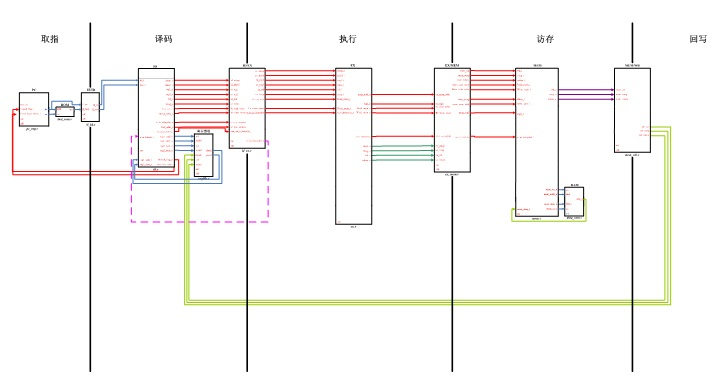
\includegraphics[width=5in]{datapath.jpg} 
\newpage

\section{流水线设计}
	\subsection{取指阶段}
	\begin{itemize}
		\item PC 模块:给出指令地址, 其中实现指令寄存器 PC,该寄存器的值就是指令地址。
		\item IF/ID模块:实现取指不译码阶段之间的寄存器,将取指阶段的结果在下一个时钟传递到译码阶段。
	\end{itemize}
	
	
	\subsection{译码阶段}
	\begin{itemize}
		\item ID 模块:对指令进行译码,译码结果包括运算类型、运算所需的源操作数、要写入的目的寄存器等。
		\item Regfile 模块:实现了 32 个 32 位通用寄存器,可以同时进行两个寄存器的读操作和一个寄存器的写操作。
		\item ID/EX 模块:实现译码不执行阶段之间的寄存器,将译码阶段的结果在下一个时钟周期传递到执行阶段。
	\end{itemize}
	
	
	\subsection{执行阶段}
	\begin{itemize}
		\item EX 模块:依据译码阶段的结果,进行指定的运算,给出运算结果。
		\item EX/MEM 模块:实现执行不访存阶段之间的寄存器,将执行阶段的结果在下一个时钟周期传递到访存阶段。
	\end{itemize}
	
	
	\subsection{访存阶段}
	\begin{itemize}
		\item MEM 模块:如果是加载、存储指令,那么会对数据存储器进行访问。
		\item MEM/WB 模块:实现访存不回写阶段之间的寄存器,将访存阶段的结果在下一个时钟周期传递到回写阶段。
	\end{itemize}


	\subsection{回写阶段}
	\begin{itemize}
		\item HILO 模块:实现寄存器 HI、LO,在乘法指令的处理过程中会使用到这两个寄存器。
	\end{itemize}
	
	
\section{冲突问题}
	因为时间等因素,没有考虑冲突的问题,只是在fibonacci数列计算的程序中可能出现冲突的两条指令之间加上了4条NOP语句。
\newpage
\section{模块接口}
	\subsection{PC模块}
	\begin{table}[!hbp]
		\centering
		\begin{tabular}{|c|c|c|c|}
		\hline
		接口名&宽度&输入/输出&作用\\
		\hline
		rst &1& 输入& 复位信号\\
		\hline
		clk &1& 输入& 时钟信号\\
		\hline
		pc &32& 输出& 要读取的指令地址\\
		\hline
		ce &1& 输出& 指令存储器使能信号\\
		\hline
		branch{\_}flag{\_}i& 1& 输入& 是否转移\\
		\hline
		branch{\_}target{\_}address{\_}i& 32& 输入& 转移地址\\
		\hline
		new{\_}pc& 32& 输入& 要读取的指令地址\\
		\hline
		\end{tabular}
	\end{table}

	\subsection{Regfile模块}
	\begin{table}[!hbp]
		\centering
		\begin{tabular}{|c|c|c|c|}
		\hline
		接口名&宽度&输入/输出&作用\\
		\hline
		rst &1& 输入& 复位信号\\
		\hline
		clk &1& 输入& 时钟信号\\
		\hline
		waddr& 32& 输出& 要写入的寄存器地址\\
		\hline
		wdata& 1& 输出& 要写入的数据\\
		\hline
		we& 1& 输入& 写使能信号\\
		\hline
		raddr1& 5& 输入& 第一个读端口地址\\
		\hline
		re1& 1& 输入& 以一个读端口使能信号\\
		\hline
		rdata1& 32& 输出& 第一个读端口的值\\
		\hline
		raddr2& 5& 输入& 第二个读端口地址\\
		\hline
		re2& 1& 输入& 以二个读端口使能信号\\
		\hline
		rdata2& 32& 输出& 第二个读端口的值\\
		\hline
		\end{tabular}
	\end{table}
	
	\newpage
	\subsection{ID模块}
	\begin{table}[!hbp]
		\centering
		\begin{tabular}{|c|c|c|c|}
		\hline
		接口名&宽度&输入/输出&作用\\
		\hline
		rst &1& 输入& 复位信号\\
		\hline
		pc{\_}i& 32& 输入& 指令地址\\
		\hline
		inst{\_}i& 32& 输入& 译码阶段指令\\
		\hline
		reg1{\_}data{\_}i& 32& 输入& 第一个读端口输入\\
		\hline
		reg2{\_}data{\_}i& 32& 输入& 第二个读端口输入\\
		\hline
		reg1{\_}read{\_}o& 1& 输出& 第一个读端口使能信号\\
		\hline
		reg2{\_}read{\_}o& 1& 输出& 第二个读端口使能信号\\
		\hline
		reg1{\_}addr{\_}o& 5& 输出& 第一个读端口地址\\
		\hline
		reg2{\_}addr{\_}o& 5& 输出& 第二个读端口地址\\
		\hline
		aluop{\_}o& 8& 输出& 运算子类型\\
		\hline
		alusel{\_}o& 3& 输出& 运算类型\\
		\hline
		reg1{\_}o &32 &输出 &源操作数1\\
		\hline
		reg2{\_}o &32 &输出 &源操作数2\\
		\hline
		wd{\_}o& 5& 输出& 目的寄存器地址\\
		\hline
		wreg{\_}o& 1& 输出& 是否需要写入目的寄存器\\
		\hline
		ex{\_}wreg{\_}i& 1& 输入& 处于执行阶段指令是否写\\
		\hline
		ex{\_}wd{\_}i& 5& 输入& 处于执行阶段指令写地址\\
		\hline
		ex{\_}wdata{\_}i& 32& 输入& 处于执行阶段指令写数据\\
		\hline
		mem{\_}wreg{\_}i& 1& 输入& 处于访存阶段指令是否写\\
		\hline
		mem{\_}wd{\_}i& 5& 输入& 处于访存阶段指令写地址\\
		\hline
		mem{\_}wdata{\_}i& 32& 输入& 处于访存阶段指令写数据\\
		\hline
		branch{\_}flag{\_}o &1& 输出& 是否转移\\
		\hline
		branch{\_}target{\_}address{\_}o& 32& 输出& 转移目标地址\\
		\hline
		is{\_}in{\_}delayslot{\_}o &1& 输出& 当前指令是否位于延迟槽\\
		\hline
		link{\_}addr{\_}o &32 &输出& 返回地址\\
		\hline
		next{\_}inst{\_}in{\_}delayslot{\_}o &1 &输出& 下一跳指令是否位于延迟槽\\
		\hline
		is{\_}in{\_}delayslot{\_}i &1 &输入 &当前指令是否位于延迟槽\\
		\hline
		\end{tabular}
	\end{table}

\newpage
	\subsection{EX模块}
	\begin{table}[!hbp]
		\centering
		\begin{tabular}{|c|c|c|c|}
		\hline
		接口名&宽度&输入/输出&作用\\
		\hline
		rst &1& 输入& 复位信号\\
		\hline
		aluop{\_}i& 8& 输入& 运算子类型\\
		\hline
		alusel{\_}i& 3& 输入& 运算类型\\
		\hline
		reg1{\_}i &32 &输入 &源操作数1\\
		\hline
		reg2{\_}i &32 &输入 &源操作数2\\
		\hline
		wd{\_}i& 5& 输入& 目的寄存器地址\\
		\hline
		wreg{\_}i& 1& 输入& 是否需要写入目的寄存器\\
		\hline
		wd{\_}o& 5& 输出& 目的寄存器地址\\
		\hline
		wreg{\_}o& 1& 输出& 是否需要写入目的寄存器\\
		\hline
		wdata{\_}o& 32& 输出& 写入目的寄存器的值\\
		\hline
		is{\_}indelayslot{\_}i& 1& 输出& 是否位于延迟槽\\
		\hline
		link{\_}address{\_}i &32& 输出& 返回地址\\
		\hline
		mem{\_}addr{\_}o& 32& 输出& 加载/存储地址\\
		\hline
		reg2{\_}o& 32& 输出& 要存的数据\\
		\hline
		\end{tabular}
	\end{table}
	
	\subsection{MEM模块}
	\begin{table}[!hbp]
		\centering
		\begin{tabular}{|c|c|c|c|}
		\hline
		接口名&宽度&输入/输出&作用\\
		\hline
		rst &1& 输入& 复位信号\\
		\hline
		wd{\_}i& 5& 输入& 目的寄存器地址\\
		\hline
		wreg{\_}i& 1& 输入& 是否需要写入目的寄存器\\
		\hline
		wdata{\_}i& 32& 输入& 目的寄存器的值\\
		\hline
		wd{\_}o& 5& 输出& 目的寄存器地址\\
		\hline
		wreg{\_}o& 1& 输出& 是否需要写入目的寄存器\\
		\hline
		wdata{\_}o& 32& 输出& 写入目的寄存器的值\\
		\hline
		reg2{\_}i &32 &输出 &要存储的数据\\
		\hline
		mem{\_}data{\_}i& 32& 输入& 读取的数据\\
		\hline
		mem{\_}addr{\_}i& 32& 输入& 加载/存储地址\\
		\hline
		is{\_}write& 1& 输出& 是否写ram\\
		\hline
		\end{tabular}
	\end{table}
\newpage
\section{监控程序}

后来目标有所修改,所以监控程序并未完成,比较有用的代码是按照原本16位term的方式打的两张32位的表。
\begin{lstlisting}[language={C++},keywordstyle=\color{blue!70},commentstyle=\color{red!50!green!50!blue!50},frame=shadowbox, rulesepcolor=\color{red!20!green!20!blue!20}] 

const AsmID RegsList[32]={
	{"zero",0},
	{"at",1},
	{"v0",2},
	{"v1",3},
	{"a0",4},
	{"a1",5},
	{"a2",6},
	{"a3",7},
	{"t0",8},
	{"t1",9},
	{"t2",10},
	{"t3",11},
	{"t4",12},
	{"t5",13},
	{"t6",14},
	{"t7",15},
	{"s0",16},
	{"s1",17},
	{"s2",18},
	{"s3",19},
	{"s4",20},
	{"s5",21},
	{"s6",22},
	{"s7",23},
	{"t8",24},
	{"t9",25},
	{"k0",26},
	{"k1",27},
	{"gp",28},
	{"sp",29},
	{"fp",30},
	{"ra",31},
};

\end{lstlisting}
\newpage
\begin{lstlisting}[language={C++},keywordstyle=\color{blue!70},commentstyle=\color{red!50!green!50!blue!50},frame=shadowbox, rulesepcolor=\color{red!20!green!20!blue!20}] 
const struct TASM const_asm[] = {
    {"AND",0X3FFF824,0XFC1FFFFF,0XFFE0FFFF,0XFFFF07FF},
    {"OR",0X3FFF825,0XFC1FFFFF,0XFFE0FFFF,0XFFFF07FF},
    {"XOR",0X3FFF826,0XFC1FFFFF,0XFFE0FFFF,0XFFFF07FF},
    {"NOR",0X3FFF827,0XFC1FFFFF,0XFFE0FFFF,0XFFFF07FF},
    
    {"ANDI",0X33FF0000,0XFC1FFFFF,0XFFE0FFFF,0XFFFF0000},
    {"XORI",0X3BFF0000,0XFC1FFFFF,0XFFE0FFFF,0XFFFF0000},
    {"LUI",0X3C1F0000,0XFFE0FFFF,0XFFFF0000,0XFFFFFFFF},
    {"ORI",0X37FF0000,0XFC1FFFFF,0XFFE0FFFF,0XFFFF0000},

    {"SLL",0X1FF800,0XFFE0FFFF,0XFFFF07FF,0XFFFFF83F},
    {"SRL",0X1FF802,0XFFE0FFFF,0XFFFF07FF,0XFFFFF83F},
    {"SRA",0X1FF802,0XFFE0FFFF,0XFFFF07FF,0XFFFFF83F},

    {"SLLV",0X3FFF804,0XFC1FFFFF,0XFFE0FFFF,0XFFFF07FF},
    {"SRLV",0X3FFF806,0XFC1FFFFF,0XFFE0FFFF,0XFFFF07FF},
    {"SRAV",0X3FFF807,0XFC1FFFFF,0XFFE0FFFF,0XFFFF07FF},

    {"MOVN",0X3FFF80B,0XFC1FFFFF,0XFFE0FFFF,0XFFFF07FF},
    {"MOVZ",0X3FFF80A,0XFC1FFFFF,0XFFE0FFFF,0XFFFF07FF},

    {"ADDU",0X3FFF821,0XFC1FFFFF,0XFFE0FFFF,0XFFFF07FF},
    {"SUBU",0X3FFF823,0XFC1FFFFF,0XFFE0FFFF,0XFFFF07FF},
    {"SLT",0X3FFF82A,0XFC1FFFFF,0XFFE0FFFF,0XFFFF07FF},
    {"SLTU",0X3FFF82B,0XFC1FFFFF,0XFFE0FFFF,0XFFFF07FF},

    {"SLTI",0X281F0000,0XFFE0FFFF,0XFFFF0000,0XFFFFFFFF},
    {"SLTIU",0X2CFF0000,0XFC1FFFFF,0XFFE0FFFF,0XFFFF0000},

    {"JR",0X3E00008,0XFC1FFFFF,0XFFFFFFFF,0XFFFFFFFF},
    {"JALR",0X3E00009,0XFC1FFFFF,0XFFFF07FF,0XFFFFFFFF},
    {"J",0X10000000,0XFC000000,0X0XFFFFFFFF,0XFFFFFFFF},
    {"JAL",0X18000000,0XFC000000,0X0XFFFFFFFF,0XFFFFFFFF},

    {"BEQ",0X13FF0000,0XFC1FFFFF,0XFFE0FFFF,0XFFFF0000},
    {"BNE",0X17FF0000,0XFC1FFFFF,0XFFE0FFFF,0XFFFF0000},

    {"BGTZ",0X1FE00000,0XFC1FFFFF,0XFFFF0000,0XFFFFFFFF},
    {"BLEZ",0X1BE00000,0XFC1FFFFF,0XFFFF0000,0XFFFFFFFF},

    {"BGEZ",0X7E10000,0XFC1FFFFF,0XFFFF0000,0XFFFFFFFF},
    {"BLTZ",0X7E00000,0XFC1FFFFF,0XFFFF0000,0XFFFFFFFF},

    {"LW",0X8FFF0000,0XFC1FFFFF,0XFFE0FFFF,0XFFFF0000},
    {"SW",0XAFFF0000,0XFC1FFFFF,0XFFE0FFFF,0XFFFF0000}
};
\end{lstlisting}

\section{收获与总结}
	通过这次大作业的实践,让我们三个对于计算机组成原理的课程有了较为完整一次复习,对于计原的那些概念性的东西有了更深的理解。
	
	
	在这次大作业的实践中让我们对于计划赶不上变化有了深刻的理解,以后在作计划的时候要一切往前并留出50\%的缓冲时间才能保证计划的顺利完成。
\end{CJK*}
\end{document}
